\begin{appendices}
% \renewcommand{\thesection}{\arabic{section}} %\Roman{section}

\addtocontents{toc}{\protect\setcounter{tocdepth}{1}}
	
	\section{Projektphasen}		
		\label{app:projektphasen_detail}
\begin{table}[H]
	\centering
	\begin{tabular}{lr}

		\rowcolor{white!15}				
		\textbf{Projekphase} & \textbf{Geplante Zeit} \\\hline

		\rowcolor{MidnightBlue!25}
	    Anforderungsanalyse & Gesamt: 7h \\\hline
	    Sichtung des Lastenhefts & 1h \\	    
	    Erstellen des Pflichtenhefts & 2h \\	    
	    Wirtschaftlichkeitsanalyse & 1h \\	     
	    Risikoanalyse & 1h \\	      
	    ''Make or Buy'' Analyse & 1h \\	    
		Anwendungsfälle definieren & 1h \\

	    \rowcolor{MidnightBlue!25}
	    Projektplanung & Gesamt: 4h \\\hline
	    Erstellen des Projektplans & 2h \\
		Erstellen des Qualitätssicherungskonzepts & 2h \\
		
		\rowcolor{MidnightBlue!25}
	    Software-Architektur & Gesamt: 14h \\\hline
	    Spezifizieren der Architekturgrundlagen & 8h \\
		Erstellen des Datenmodells & 4h \\
		Erstellen des Testkonzepts & 2h \\
		
		\rowcolor{MidnightBlue!25}
	    Implementierung & Gesamt: 26h \\\hline
	    Erstellen der Datenbanktabellen & 2h \\
		Entwicklung des Backends & 7h \\
		Entwicklung des Frontends & 9h \\
		Dokumentation des Quellcodes & 2h \\
	    Testing & 2h \\
		Soll-Ist-Vergleich & 2h \\
		Puffer für Korrekturen & 2h \\
		
		\rowcolor{MidnightBlue!25}
	    Projektabschluss & Gesamt: 3h \\\hline
	    Anwenderschulung & 2h \\
		Abnahme & 1h \\
		
		\rowcolor{MidnightBlue!25}
	    Sonstiges & Gesamt: 16h \\\hline
	    Projektdokumentation & 12h \\
		Allgemeiner Puffer & 4h \\\hline
		
		\textbf{Gesamt} & \textbf{70h}				
			    
	\end{tabular}
	\caption{Projektphasen detailliert}
	\label{tab:projektphasen_detail}
	\end{table}
		\newpage

	\section{Risikoanalyse}		
		\label{app:risikoanalyse}

	\begin{longtable}{
		p{\dimexpr 0.2\linewidth-2\tabcolsep} |
		p{\dimexpr 0.2\linewidth-2\tabcolsep} |
		p{\dimexpr 0.2\linewidth-2\tabcolsep} |
		p{\dimexpr 0.2\linewidth-2\tabcolsep} |
		p{\dimexpr 0.2\linewidth-2\tabcolsep}
	}

		\rowcolor{white!15}				
		\textbf{Risiko} & \textbf{Ursache} & \textbf{Maßnahme} & \textbf{Eintrittswahr. nach der Maßnahme} & \textbf{Auswirkung nach der Maßnahme} \\\endhead\hline

	
		\rowcolor{MidnightBlue!25}
		\multicolumn{5}{c}{Terminrisiken} \\\hline
		Nicht einhalten des Abnahmetermins & uneingeplante Hindernisse & keine & mittel & Start der Anwendungsnutzung verzögert sich \\
		
		\rowcolor{MidnightBlue!25}
		\multicolumn{5}{c}{Technische Risiken} \\\hline
		Anwendung ist auf Zielplattform nicht lauffähig & Entwicklung gegen falsche Plattform & Anpassung der Anwendung & mittel & Zustäzlicher Zeitbedarf für Anpassungen \\
		
		\rowcolor{MidnightBlue!25}
		\multicolumn{5}{c}{Personelle Risiken} \\\hline
		Ausfall des Projektleiters & Krankheit & keine & gering & Projekt kommt zum erliegen \\		
		Ausfall eines Projektmitarbeiters & Krankheit & keine & gering & Projekt kommt zum erliegen \\
						
		\rowcolor{MidnightBlue!25}
		\multicolumn{5}{c}{Planungsrisiken} \\\hline
		Unterschätzung der Dauer einzelner Phasen & mangelnde Erfahrung & nachtrgäliche Planung & mittel & Verzögerung des Projektabschluss \\
		Auslassung relevanter Phasen & mangelnde Erfahrung & nachträgliche Planung & gering & Verzögerung des Projektabschluss \\
		
		\rowcolor{MidnightBlue!25}
		\multicolumn{5}{c}{Risiken der Analyse und Konzeption} \\\hline
		Fehlerhafte Ist-Analyse & ungenaue Analyse & Nachbesserung d. Analyse & gering & iterativer Rücksprung im Entwicklungsprozess \\
		Fehlerhafte Soll-Analyse & fehlerhafte Spezifikation & Nachbesserung d. Analyse & gering & iterativer Rücksprung im Entwicklungsprozess \\
		Fehlerhafte Architektur / Konzept & ungenaue Spezifikation & Neukonzeption & gering & iterativer Rücksprung im Entwicklungsprozess \\
		
		\rowcolor{MidnightBlue!25}
		\multicolumn{5}{c}{Realisierungrisiken} \\\hline
		Unerwartete Entwicklungsprobleme & nicht bestimmbar & teilweise NeuKonzeption & mittel & verlängte Entwicklungszeit \\
		
		\rowcolor{MidnightBlue!25}
		\multicolumn{5}{c}{Betreuungs- und Wartungsrisiken} \\\hline
		Breaking-Changes & MediaWiki Update & Anpassung der Geschäftslogik & hoch & keine \\
	    
	
	\caption{Risikoanalyse detailliert}
	\label{tab:risikoanalyse_detail}	
\end{longtable}
	

		\newpage		
		
	\section{''Make or Buy''-Bewertung}		
		\label{app:make_or_buy}

Grundlage der im Folgenden betrachteten Alternativen ist eine umfängliche Recherche bezüglich der Kernfrage
''Welche Lösungen zur Erstellung von Handbüchern aus Wikis existieren bereits?''.
Betrachtet werden hier nur die stärksten Ergebnisse dieser Recherche, um die Übersichtlichkeit der Analyse zu bewahren.

\begin{table}[H]
	\centering
	\begin{tabular}{lcc}

		\rowcolor{white!15}				
		\textbf{Alternative} & \textbf{Nutzen} & \textbf{Wirtschaftlichkeit} \\\hline		
		
		\rowcolor{MidnightBlue!15}
		MediaWiki Erweiterung 								& 					& 							\\\hline
		\hspace{1.5em} einfache Installation 				&					& $\oplus$  				\\
		\hspace{1.5em} Installation für jedes Wiki nötig 	&					& $\ominus$ 				\\
		\hspace{1.5em} Workflow umständlich 				& $\ominus$ 		& $\ominus$ 				\\
		\hspace{1.5em} Ergebnis bedarf händische Anpassung	& $\ominus\ominus$	& $\ominus\ominus$ 			\\
		\hspace{1.5em} Komptibilitätsprobleme mit MediaWiki	&  					& $\ominus$ 				\\
		
		\rowcolor{MidnightBlue!15}
		Erstellung der Anwendung durch Dienstleister 		& 					& 							\\\hline
		\hspace{1.5em} spezialisierte Anwendung 			& $\oplus\oplus$	& $\ominus\ominus\ominus$	\\
		\hspace{1.5em} Wartung durch Dienstleister nötig 	&					& $\ominus\ominus$ 			\\
		\hspace{1.5em} Risikoauslagerung 					&  					& $\oplus\oplus$ 			\\
		
		\rowcolor{MidnightBlue!15}
		Eigenständige Erstellung der Anwendung 				& 					& 							\\\hline
		\hspace{1.5em} spezialisierte Anwendung 			& $\oplus\oplus$	& $\ominus\ominus$ 			\\
		\hspace{1.5em} Wartung durch eigene Mitarbeiter  	& $\oplus$			& $\oplus$ 					\\
		\hspace{1.5em} Tragen von Risiken 					&  					& $\ominus$ 				\\									
			    
	\end{tabular}
	
	\caption{Detaillierte ''Make or Buy''-Bewertung}
	\label{tab:make_or_buy_detail}
\end{table}		
		\newpage
	
	\section{Kostenübersicht nach Projektphasen}		
		\label{app:kosten}

Grundlage der Folgenden Kostenübersicht sind die in Anhang \ref{app:projektphasen_detail} aufgeführten Phasen des Projekts.
Als Rechnungsgrundlage wird der in Kapitel \ref{sec:wirtschaftlichkeitsanalyse} ermittelte Stundensatz von 17 \euro{} herangezogen.

\begin{table}[H]
	\centering
	\begin{tabular}{lr}

		\rowcolor{white!15}				
		\textbf{Phase} & \textbf{Kosten}  \\\hline		
		
		
		Anforderungsanalyse		& 119 \euro \\
		Projektplanung			& 68 \euro \\
		Software-Architektur	& 238 \euro \\
		Implementierung			& 442 \euro \\
		Projektabschluss		& 51 \euro \\
		Sonstiges				& 272 \euro \\\hline
		\textbf{Gesamt}			& \textbf{1190 \euro}
		
			    
	\end{tabular}
	
	\caption{Kosten unterteilt nach Projektphasen}
	\label{tab:kosten_detail}
\end{table}		
		\newpage

	\section{Nutzwertanalyse}		
		\label{app:nutzwertanalyse}

\subsubsection{Backend-Architektur}

Im Folgenden wird über eine Nutzwertanalyse die beste Backend-Architektur ausgewählt.
Die hier betrachteten Alternativen sind die stärksten Ergebnisse einer vorangegangen Recherche. 

\begin{savenotes}
\begin{table}[H]
	\centering
	\begin{tabular}{lcccc}

		\rowcolor{white!15}				
		\textbf{Eigenschaft} 			& \textbf{Gewichtung}
			& \textbf{JEE-Stack\footnote{\url{http://www.oracle.com/technetwork/java/javaee/overview/index.html}, abgerufen am 08.11.2015}}
			& \textbf{GNS-Framework\footnote{ein betriebsinternes Framework zur entwicklung von Webanwendungen}}
			& \textbf{SrpingMVC\footnote{\url{https://spring.io}, abgerufen am 08.11.2015}} \\\hline		
		
		REST-Api integriert				& 3						& 5						& 0							& 4 \\
		\pbox{4cm}{Trennung von \\ Back- und Frontend}	& 4						& 5						& 0							& 4 \\						
		Dokumentation					& 2						& 3						& 1							& 5 \\
		Testbarkeit						& 2						& 2						& 1							& 3 \\
		\pbox{4cm}{Refactoring \\(ggf. durch Dritte)}	& 3						& 3						& 4							& 2 \\
		
		\rowcolor{MidnightBlue!15}
		\textbf{Gesamt}				& \textbf{14}			& \textbf{18}			& \textbf{6}				& \textbf{18} \\\hline
		\rowcolor{white!15}				
		\textbf{Nutzwert} 				& 						& \textbf{3,86}			& \textbf{1,14} 			& \textbf{3,57} \\
											
			    
	\end{tabular}
	
	\caption{Detaillierte Nutzwertanalyse bezüglich der Backend-Architektur}
	\label{tab:nutzwertanalyse_backend}
\end{table}
\end{savenotes}


\subsubsection{Frontend-Architektur}

Im Folgenden wird über eine Nutzwertanalyse die beste Frontend-Architektur ausgewählt.
Die hier betrachteten Alternativen sind die stärksten Ergebnisse einer vorangegangen Recherche. 

\begin{savenotes}
\begin{table}[H]
	\centering
	\begin{tabular}{lccccc}

		\rowcolor{white!15}				
		\textbf{Eigenschaft}	& \textbf{Gewichtung}
			& \textbf{JSF\footnote{\url{http://www.oracle.com/technetwork/java/javaee/javaserverfaces-139869.html}, abgerufen am 08.11.2015}}
			& \textbf{Angular\footnote{\url{https://angularjs.org}, abgerufen am 08.11.2015}}
			& \textbf{kein Framework}
			& \textbf{React\footnote{\url{https://facebook.github.io/react/}, abgerufen am 08.11.2015}} \\\hline		
		
		Bootstrap-Aufwand		& 2						& 3				& 3					& 5							& 2 \\
		Modularität				& 4						& 4				& 3					& 1							& 5 \\						
		Erweiterbarkeit			& 5						& 3				& 4					& 0 						& 5 \\
		Dokumentation			& 2						& 3				& 5					& 4 						& 4 \\
		User-Experience			& 4						& 3				& 5					& 2 						& 5 \\
		Kompatibilität			& 2						& 4				& 2					& 5 						& 2 \\
		
		\rowcolor{MidnightBlue!15}
		\textbf{Gesamt}			& \textbf{19}			& \textbf{20}	& \textbf{22}		& \textbf{17}				& \textbf{23} \\\hline
		\rowcolor{white!15}				
		\textbf{Nutzwert} 		& 						& \textbf{3,32}	& \textbf{3,79} 	& \textbf{2,11} 			& \textbf{4,26}\\
											
			    
	\end{tabular}
	
	\caption{Detaillierte Nutzwertanalyse bezüglich der Frontend-Architektur}
	\label{tab:nutzwertanalyse_frontend}
\end{table}
\end{savenotes}
		\newpage
		
	\section{Use-Case-Diagramme}		
		\label{app:use_case_diagramm}

	\subsection{Wiki konvertieren}
	\begin{center}
	\begin{figure}
	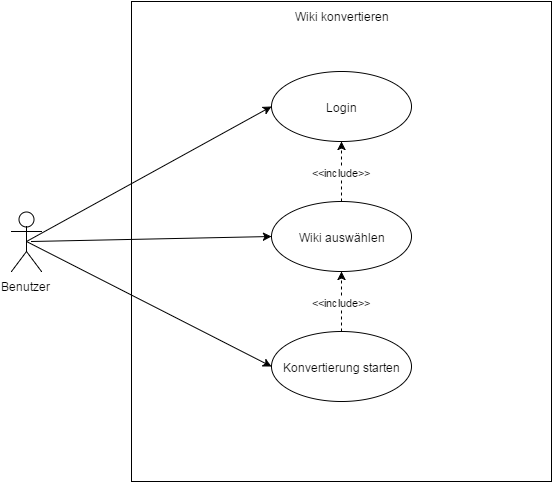
\includegraphics[width=0.85\textwidth]{images/UC_wiki_konvertieren}	
	\caption{Use-Case ''Wiki konvertieren''}
	\end{figure}
	\end{center}
	
	\subsection{Wiki bearbeiten}
	\begin{center}
	\begin{figure}
	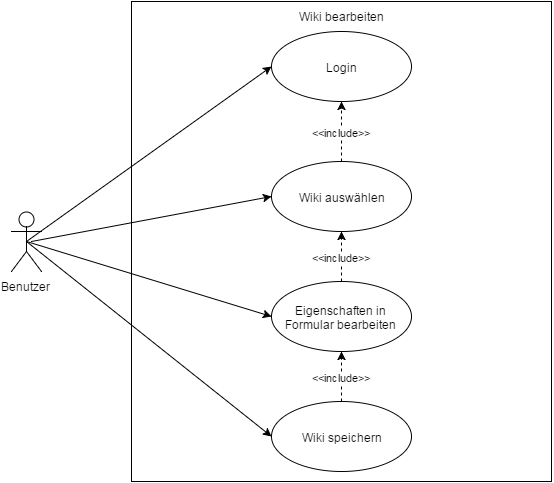
\includegraphics[width=0.85\textwidth]{images/UC_wiki_bearbeiten}	
	\caption{Use-Case ''Wiki bearbeiten''}
	\end{figure}
	\end{center}
		\newpage		
		
	\section{Qualitätsanforderungen (Auszuf aus Pflichtenheft)}		
		\label{app:qualitaetsanforderungen}

\begin{table}[H]
	\centering
	\begin{tabular}{lcccc}
		\rowcolor{white!15}
		\textbf{Qualitätsmerkmal}			& \textbf{sehr gut}	& \textbf{gut}	& \textbf{normal}	& \textbf{nicht relevant}	\\\hline
		
		\rowcolor{MidnightBlue!15}
		Funktionalität 						&					&				&					&							\\
		\hspace{1.5em} Angemessenheit		&					&				& X					&							\\
		\hspace{1.5em} Richtigkeit			&					&	X			& 					&							\\
		\hspace{1.5em} Interoperabilität	&	X				&				& 					&							\\
		\hspace{1.5em} Sicherheit			&					&	X			& 					&							\\
		\hspace{1.5em} Ordnungsmäßigkeit	&					&				& X					&							\\
		\hspace{1.5em} Konformität			&					&				& X					&							\\
		
		\rowcolor{MidnightBlue!15}
		Zuverlässigkeit 					&					&				&					&							\\
		\hspace{1.5em} Reife				&					&				& X					&							\\
		\hspace{1.5em} Fehlertoleranz		&					&				& X					&							\\
		\hspace{1.5em} Wiederherstellbarkeit&					&	X			& 					&							\\
		\hspace{1.5em} Konformität			&					&				& X					&							\\
		
		\rowcolor{MidnightBlue!15}
		Benutzbarkeit 						&					&				&					&							\\
		\hspace{1.5em} Verständlichkeit		&	X				&				& 					&							\\
		\hspace{1.5em} Erlernbarkeit		&					&	X			& 					&							\\
		\hspace{1.5em} Bedienbarkeit		&					&	X			& 					&							\\
		\hspace{1.5em} Attraktivität		&					&				& X					&							\\
		\hspace{1.5em} Konformität			&					&				& 					&	X						\\
		
		\rowcolor{MidnightBlue!15}
		Effizienz	 						&					&				&					&							\\
		\hspace{1.5em} Zeitverhalten		&					&	X			& 					&							\\
		\hspace{1.5em} Verbrauchsverhalten	&					&				& X					&							\\		
		\hspace{1.5em} Konformität			&					&				& X					&							\\
		
		\rowcolor{MidnightBlue!15}
		Wartbarkeit 						&					&				&					&							\\
		\hspace{1.5em} Analysierbarkeit		&					&				& X					&							\\
		\hspace{1.5em} Modifizierbarkeit	&					&	X			& 					&							\\
		\hspace{1.5em} Stabilität			&					&				& X					&							\\
		\hspace{1.5em} Testbarkeit			&					&				& 					&	X						\\		
		\hspace{1.5em} Konformität			&					&				& X					&							\\
		
		\rowcolor{MidnightBlue!15}
		Übertragbarkeit 					&					&				&					&							\\
		\hspace{1.5em} Anpassbarkeit		&					&	X			& 					&							\\
		\hspace{1.5em} Installierbarkeit	&					&	X			& 					&							\\
		\hspace{1.5em} Koexistenz			&	X				&				& 					&							\\
		\hspace{1.5em} Austauschbarkeit		&					&	X			& 					&							\\		
		\hspace{1.5em} Konformität			&					&				& 					&	X						\\
		
	
	\end{tabular}
	\caption{Qualitätsanforderungen an die Anwendung detailliert}
	\label{tab:qualitaetsanforderungen}
\end{table}
		\newpage
		
	\section{Lastenheft (Auszug)}
		\label{app:lastenehft}

\subsubsection*{Zielbestimmung}

	\paragraph*{Musskriterien}
		\begin{itemize}
			\item Benutzerverwaltung
			\begin{itemize}
				\item Benutzer anlegen
				\item Benutzerdaten editieren
				\item Benutzer löschen
			\end{itemize}
			\item Wikiverwaltung
			\begin{itemize}
				\item Wiki anlegen
				\item Wikidaten editieren
				\item Wiki löschen
				\item Handbuch aus Wiki generieren
				\item Handbuch runterladen
			\end{itemize}
		\end{itemize}

	\paragraph*{Wunschkriterien}
		\begin{itemize}
			\item Handbuchversionen
			\begin{itemize}
				\item Handbuchhistorie eines Wikis einsehen
				\item Handbuch aus Historie löschen
				\item Älteres Handbuch runterladen
			\end{itemize}
			\item Handbuchgenerierung
			\begin{itemize}
				\item Aktuellen Fortschritt während Generierung anzeigen
				\item Erstellung für Wikis sperren, wäend aktuelle Generierung läuft
			\end{itemize}
			\item Gruppenverwaltung
			\begin{itemize}
				\item Gruppen anlegen
				\item Gruppen löschen
				\item Benutzer Gruppen zuteilen
				\item Rechte Gruppen zuteilen
			\end{itemize}
		\end{itemize}

	\paragraph*{Abgrenzungskriterien}
		\begin{itemize}
			\item Single-Sign-On über GNS internes ActiveDirectory
			\item Anlegen / Konfigurieren der Laufzeitumgebung innerhalb der GNS DMZ
		\end{itemize}

\subsubsection*{Produkteinsatz}

	\paragraph*{Anwendungsbereiche}
		Technischer/administrativer Anwendungsbereich.

	\paragraph*{Zielgruppen}
		Die Zielgruppe besteht ausschließlich aus Mitarbeitern der GNS mbH.
		Vornehmlich wird das Produkt durch Angestellte der Abteilung KIS benutzt werden.

	\paragraph*{Betriebsbedingungen}
		Das Produkt wird als Webanwendung bereitgestellt. Das Produkt ist über das Internet erreichbar.
		Es wird eine Up-Time von nahezu 100\% angestrebt.


\subsubsection*{Produktübersicht}
	Das Produkt ist eine Webapplikation, welche es dem Benutzer erlaubt den Inhalt eines existierenden
	Mediawikis in eine PDF- respektive HTML-Datei zu konvertieren und diese anschließend herunterzuladen.
	Hierzu kann der Nutzer selbstständig neue Wikis indizieren um diese für das spätere Konvertieren
	bereitzustellen. Konvertierte Mediawikis können anderen Benutzern ebenfalls zum download bereitgestellt
	werden.
		\newpage
		
\section{Oberflächenprototyp}
		\label{app:prototyp}
		
	\begin{figure}[H]
	\begin{center}
	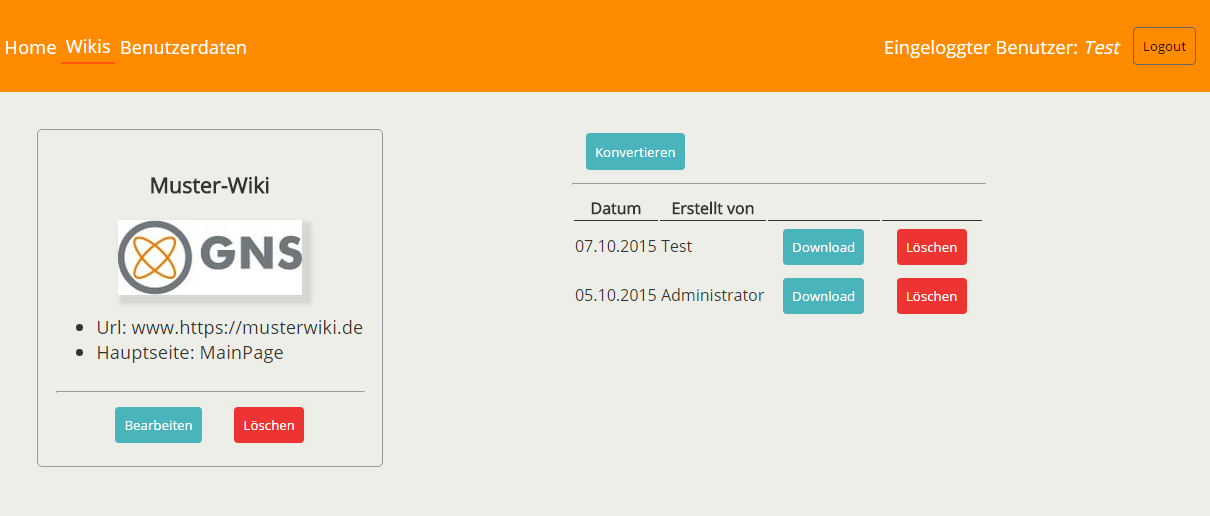
\includegraphics[width=0.85\textwidth]{images/prototyp1}	
	\caption{Prototyp - Layout für Desktop-Browser}
	\end{center}
	\end{figure}
			
	\begin{figure}[H]
	\begin{center}
	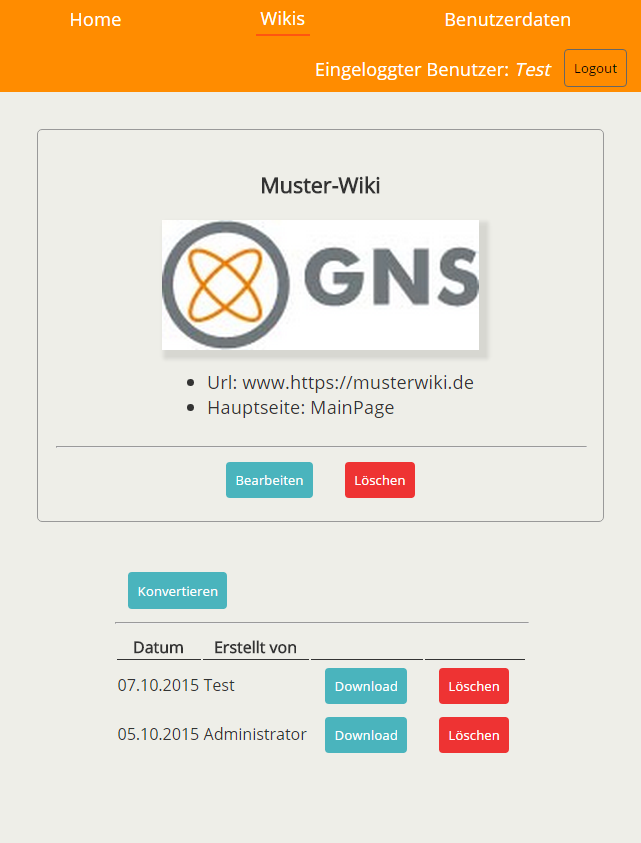
\includegraphics[width=0.85\textwidth]{images/prototyp2}	
	\caption{Prototyp - Layout für Mobile-Browser}
	\end{center}
	\end{figure}
	
		\newpage
		
\end{appendices}